\chapter{Design}

The goal is to create a C-like language which then compiles down to GPIR code.
The language should be as C-like as possible ideally it should be as much
of a complete subset of C++ as possible.

C++ is a statically typed, imperative language which is sequentially evaluated by default.
GPIR is a dynamically typed functional language which is evaluated in parallel by default.
These two languages use two completely different paradigms, so the language design has to 
ensure that GPC is like C++ and can be compiled to GPIR without too much trouble.

\section{GPC Language Design Decisions}
\label{sec:Lang}

\subsection{Parallel Evaluation}
GPIR is parallel evaluated by default, with a \texttt{seq} function which
evaluates the given arguments in sequential order. Mapping GPC code into
GPIR code which can be evaluated in parallel should be possible, and allows
GPC to take advantage of parallel evaluation by default. GPC should also
have a method of sequentially evaluation of multiple statements.


\subsection{Serial Semantics}
Having serial semantics is helpful to the programmer as it makes
it easy to reason about the behaviour of parallel code.
This is due to the ability to run the entire parallel code in a single
thread as if it were sequential code. 

\subsection{Purely Functional}

In the GPRM jumping to labels is an expensive operation, to avoid
this function calls will need to be inlined, and loops unrolled 
as much as possible. The execution path will also need to be known 
during compile time to achieve this. 

Another one of the major benefits of being able to compute the execution
path at runtime is that recursive functions can be more efficiently parralelised
by the compiler. The following Mergesort example is used to illustrate this.

\begin{lstlisting}[style=myGPC]

//Use Sort class from Kernel
GPRM::Kernel::Sort MS;

int size = 8

void merge_sort(int *a, int low, int high) {
    if (low + 1 < high) {
        mid = (low + high) / 2;
   
        seq {
            par {
                merge_sort(a, low, mid);
                merge_sort(a, mid, high);
            }
            MS.merge(a, low, mid, high);            
        }
    
)

void GPC_merge_sort(int *a) {
    merge_sort(a, 0, size);
}

\end{lstlisting}

The merge kernel calls be be reduced down to a tree:

\begin{center}
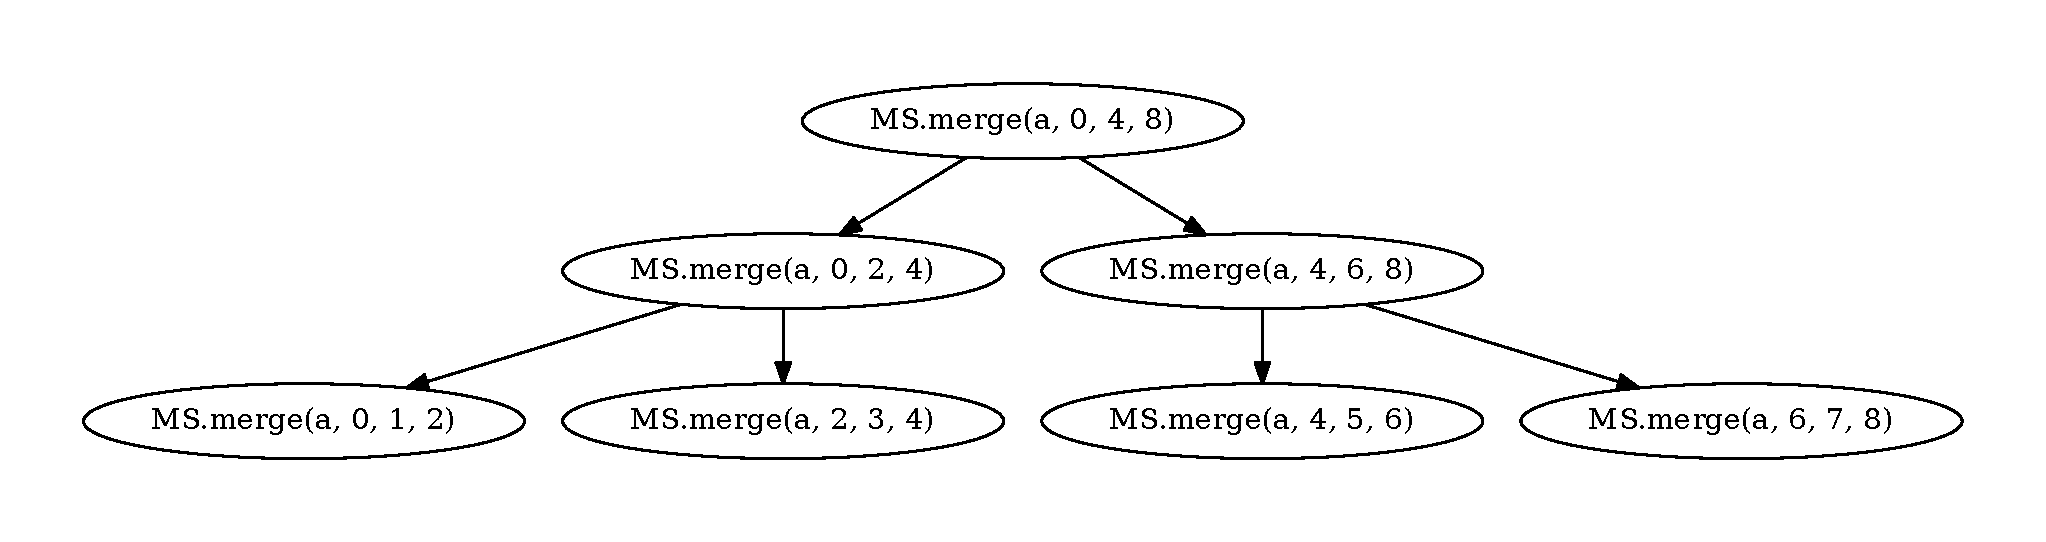
\includegraphics[scale=0.5]{graphs/mergesortTree.pdf}
\end{center}


From the bottom up, the merge operations in the row can be performed in
parallel, knowing the execution path at compile time allows for the compiler
to map these to seperate threads. 


However if the language is Turing-complete deciding the execution path
of a given program is essentially the Halting Problem. It has been proven that the solution to this problem is undecidable\cite{halting} 

To avoid this problem, the language needs to be restricted to a point where it can still be useful and the execution
path decided at compile time.

If the language is purely functional with no side effects then this avoids the problem, however a program
with no side effects is useless. There is one major feature that must ne in the language that invokes
side effects which is method calls for kernel objects. 

Enforcing that anything returned from a kernel object method call's type then has to be in the 
\texttt{GPRM::Kernel} namespace, and anything passed into a kernel object method call must be in the GPRM::Kernel
namespace. This allows passing impure values between kernel methods but restricts them being used
for conditional statements. Essentially we still have side effects but they're restricted to
only being in Kernel space and not in the GPRM. The execution of GPC code is then purely functional
and the execution path of code can be determined at compile time without oo much difficulty.

\section{GPC Language Features}

    This section explains the features of the language with respect to the design decisions in section ~\ref{sec:Lang}.

\subsection{Syntax}
        The syntax aims to be as close to C/C++ as possible. Statements must end with a semicolon. 
        All variables must be statically typed. Blocks are surrounded in braces. Case sensitivity
        will be enforced.

\subsection{New Operators}
        Two new operators not currently present in C++ \texttt{seq} and \texttt{par} are introduced. 
        These are placed before a block
        of statements to determine whether each individual statement within the block are
        to be evaluated in sequential or parallel. By default a block of statements are evaluated
        in parallel, but the par keyword makes it more explicit especially if there's lots of nested
        seq/par blocks.

\subsection{Objects}
Objects can be declared in the top level scope, and must be in the GPRM::Kernel namespace.
For example declaring a test object from a class called Test in the \texttt{GPRM Kernel} namespace:

\begin{lstlisting}[style=myGPC]
GPRM::Kernel::Test test;
\end{lstlisting}

Standard C++ method calling syntax can be applied to objects.
\begin{lstlisting}[style=myGPC]
test.m1();
\end{lstlisting}



\subsection{Compatibility with C++}
Making the language completely compatible with C++ in that all GPC code can be
compiled with a C++11 compatible compiler allows programers that are familiar to
C++ write GPC code with little difficulty. As long as they are aware of the restrictions
that GPC has compared to C++. However the new keywords \texttt{seq} and \texttt{par} are not in the language.

Currently preprocessor directives aren't supported in GPC so the compiler can
just ignore lines starting with \texttt{"\#"}, and define \texttt{seq} and \texttt{par} as no-ops. 
For example this snippet of code compiles with both the GPC compiler and 
C++ compilers:

\begin{lstlisting}[style=myGPC]
#include "GPRM/Kernel/Test.h"
#define seq
#define par

GPRM::Kernel::Test test;

int entry_fn() {
    seq {
        int a = test.m1();
        int b = test.m2(a);        
        par {
            test.m3(b);
            test.m3(b + 1);
        }
        return 0;
    }
}
\end{lstlisting}

When this code is compiled with a C++ compiler it will removed the seq and par
keywords and what will be left is plain blocks. Essentially this should generate a
serial version of the program which should generate the exact same results
as the version compiled by GPC and run on the GPRM. This supports the 
design decision of serial semantics.

This is useful for implementing the compiler as it allows for
testing that the code generated by GPC is generating the correct results
by comparing it to the C++ version. It also allows for easier porting of
programs already written in C++ to GPC. Programers can use tools
already made for C++ to debug their serial code before attempting
to run it in parallel on the GPRM.

\subsection{Types}
        C++ types such as string, char, bool, int, and double are included.
        Pointers, and "multilevel" pointer types are included (e.g. int**, char*).
        However pointers are restricted in that you cannot take
        an address of any variable, adding and subtracting integers
        from pointers is allowed. Usually pointers are passed into
        the GPRM from the C++ caller to represent an Array.

        return values from kernel method calls are implicitly placed
        in the \texttt{GPRM::Kernel} namespace. 

For example:

\begin{lstlisting}[style=myGPC]
int x = obj.method(5);
\end{lstlisting}

This is implicitly cast to:

\begin{lstlisting}[style=myGPC]
GPRM::Kernel::int x = obj.method(5);
\end{lstlisting}     

If a binary expression involved a Kernel value and a "pure" value
then the "pure" value is implicitly upcast before the operation takes
place. For example:

\begin{lstlisting}[style=myGPC]
bool y = obj.m1(10) == 5;    
\end{lstlisting}

is implicitly cast to:

\begin{lstlisting}[style=myGPC]
GPRM::Kernel::bool y = ob.m1(10) == 5;
\end{lstlisting}

This feature stops impurity in the GPC code execution, as the type system
should be able to stop Kernel types being used in conditional
statements. 

For example this is not allowed:
\begin{lstlisting}[style=myGPC]

seq {
    int x = obj.method(5);
    if (x == 10) {
        //Do Stuff
    }    
}

\end{lstlisting}

If statements must take a "pure" boolean type as its conditional.
x == 10 is a GPRM::Kernel::bool type, so this raises a type error.
  
\subsection{Operations}
        Most basic binary arithmetic operations are included i.e. 
        (+, -, *, /, \%, ==, !=, \&\&, $||$ , \lstinline|<<|, \lstinline|>>|, \lstinline|&|, $|$, 
        \lstinline|^|) as well as
        unary operations 
        (\lstinline|-|, \lstinline|~|, \lstinline|!|).

        (+=, ++, --, -=) are not included, due to the single assignment rule.
        Although an exception is made for the "afterthought" of the for loop construct, in which
        the integer loop variable can be incremented with += or decremented by -=.

\subsection{Functions}
        Function syntax is exactly the same as C. 


\subsection{Single assignment}
Variables in GPC can only be assigned once per scope.

for example the following isn't allowed:

\begin{lstlisting}[style=myGPC]
int i = 0;
int i = i + 1;
\end{lstlisting}

Since \texttt{i} is already in scope, it cannot be redefined in the same scope.

The following code is allowed:

\begin{lstlisting}[style=myGPC]
int i = 0;
{
   int i = i;
}
\end{lstlisting}

Since \texttt{i} inside the block is declared in a new scope.

Also variables must be assigned when they are declared, for example the following is not allowed:

\begin{lstlisting}[style=myGPC]
int x;
x = 5;
\end{lstlisting}

\subsection{For-Loops}
For loops have the same syntax as C/C++ for loops with some restrictions:

\begin{itemize}
\item There is a single loop variable which must be declared inside the loop, and must be an integer.

\item The conditional expression must result in a "pure" boolean type, a \textit{GPRM::Kernel::bool}
     type is not allowed.

\item The "afterthought" of the for loop must consist of the loop variable with either the \texttt{+=} operator
      or \texttt{-=} operator with a "pure" integer value on the right hand side. This is the only place these
      binary operations are allowed to occur in a GPC program. 

\end{itemize}

These restrictions and properties are in place to keep the functional "purity" of GPC code,
allowing complete compatibility with the C++ language, and keeps the property of GPC programs
having serial semantics.  
At compile time the loop is fully unrolled, these restrictions also allow for detection
at compile time whether or not the loop is infinite.  

It's worth noting that these restrictions are similar to the restrictions on the \textit{cilk\_for} loop.
The \textit{cilk\_for} loop must declare a single initial loop variable, the conditional expression must 
compare the loop variable with a constant "termination expression", and the "afterthought" must either increment
or decrement the loop variable by some amount.
\cite{cilkfor}

An example of a for loop is as follows:


\begin{lstlisting}[style=myGPC]
for(int i = 0; i < 5; i+=1) {
    obj.m1(i);
}
\end{lstlisting}


During compilation this loop is fully unrolled and is equivalent
to the following:

\begin{lstlisting}[style=myGPC]
par {
    obj.m1(0);
    obj.m1(1);
    obj.m1(2);
    obj.m1(3);
    obj.m1(4);
}
\end{lstlisting}


\subsection{Top Level Statement Restrictions}
Top Level statements are restricted to being either object declarations, function definitions,
or constant variable assignments. This is partly to be like C++ and also to remove any ambiguity
on how top level statements are evaluated.


\subsection{Entry Function}
Since the GPIR function is called by C++ code, it's not preferrable to name the function "main".
Also the C++ code may be calling more than one GPIR function during its lifetime so a static
name is also not preferable. The GPIR code entry function has the same name as the GPC source
file it is in. For example the entry function  for "test.gpc" would be called "test". This method
of determining an entry function is not ideal, but is easy to change in the future if needed.





